\chapter{Summary}\label{ch:summary}
The following chapter concludes the thesis by summarizing its results and the framework's limitations. Furthermore, an outlook on the framework's source code availability and possible future changes will be given.

\section{Limitations}
The framework given in this thesis tries to not restrict any \uima{} related features. To achieve this in combination with thread-safety, each pipeline is separated into their own \jvm{}, guaranteeing maximal isolation. This however, can be unwanted, since Analysis Engines can no longer interact with each other by native Java \lstinline|Thread| logic or static variables. 

The \lstinline|AnalysisResult| object, returned by the \spark{} cluster wraps around a \lstinline|JavaRDD| and delegates the logic to it. However, it restricts the user from directly accessing the \spark{} \api{} by setting the underlying \rdd{} to private. This is done to isolate the user from having to handle \spark{} related concepts, but prevents further processing inside the cluster before collecting the data first. The framework can easily be extended to provide such functionality though, as explained in Section~\ref{sec:outlook}. 


\section{Related Work}
\label{sec:related}
Taking effort to scale \uima{} has been done numerous times. The most prominent result was the implementation of the question answering system Watson \cite{epstein2012making}. This approach used native \uimaas{}, although the engineers changed the \uimaas{} source code themselves. Other approaches that are trying to be generic solutions while not posing too many restrictions or being too intrusive into the native \uima{} concepts or even code, are Leo and v3NLP.
\subsection{Leo}
\label{ssec:leo}
The Leo framework was developed by \vinci{} to allow for the easy deployment of annotators in an \uimaas{} environment \cite{leo}. Since it wraps around most concepts of \uima{} and \uimaas{}, its architecture closely resembles \uimaas{}. This can be seen in Figure~\ref{fig:leo}. Given a number of instances of \lstinline|LeoAEDescriptor|, which are compatible with the native \uima{} Analysis Engine, Leo is able to automatically write an \uimaas{} deployment descriptor file and use it to deploy a \lstinline|Service| instance. This also is just a wrapper around \uimaas{} native service, which tries to register to a given broker implementation. Leo does not provide a broker implementation by its own, but depends on an existing \uimaas{} installation, which in turn provides ActiveMQ, as described further in Section~\ref{ssec:uimaas}.
\begin{figure}[hbt]
	\centering
	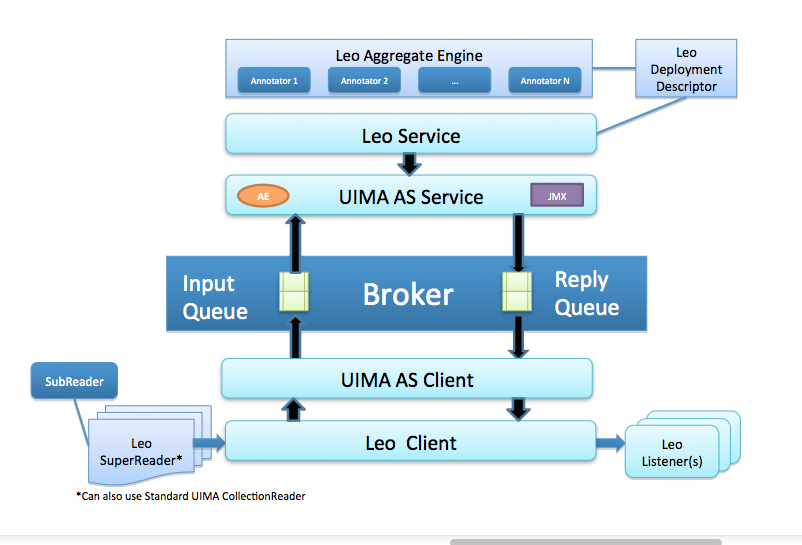
\includegraphics[width=1\textwidth]{leo}
	\caption[The Leo architecture wrapping around UIMA-AS.]{The Leo architecture wrapping around \uimaas{} \cite{leo}}
	\label{fig:leo}
\end{figure}
Given such an instance of a broker-service architecture, Leo is now able to perform requests to said broker. The Leo \lstinline|Client| class provides access to the native \uimaas{} capability of querying the services for analysis results. For this, Leo utilizes the class \lstinline|LeoCollectionReader|, which also is just a wrapper around the native \uima{} Collection Readers and can be easily converted to one and vice versa.

The Leo source code repository\footurl{https://github.com/department-of-veterans-affairs/Leo}{2018-09-14} shows that the last change was in January 2018, without providing any comments or history\footurl{https://github.com/department-of-veterans-affairs/Leo/commit/038f7d5c542fa564c2997403769943ac47638692}{2018-09-14}. This, and the fact that the project only has four contributors and no pull request as of the time of writing shows that the Leo framework project is not well-maintained.

A static code analysis with FindBugs\footurl{http://findbugs.sourceforge.net/}{2018-09-14} on the current source code\footnote{Commit 038f7d5c542fa564c2997403769943ac47638692 on 2018-09-14} shows 29 potential bugs, of which seven are rated as `scary' by FindBugs. Another code analysis tool, SonarLint\footurl{https://www.sonarlint.org/}{2018-09-14} which also checks the coding style found a total of 626 bugs, vulnerabilities and code smells. 

\subsection{v3NLP}
The framework v3NLP was first introduced in 2011 by Divita and Trietler in \cite{divita2011finding} as a successor to HITEx\footnote{Health Information Text Extraction}. Both, HITEx and v3NLP were initially built on top of the Gate framework but have switched to \uima{} since. v3NLP provides capabilities to process \nlp{} tasks especially in the medical field. It is therefore influenced by the context of a medical environment. It provides 34 pre-composed pipelines, all related to clinical text analysis. However, it enforces the use of the CHIR\footnote{Consortium for Healthcare Informatics Research} Common Model, which is an ontology of labels from already existing \nlp{} systems. This model is encoded in a default type system the framework is using and it can be extended at will. This is supposed to ensure interoperability between different \nlp{} components that were developed for v3NLP. Notice that this poses a restriction on the user of the framework, since they are forced to always include this type system \cite{divita2016v3nlp}. The framework also provides scaling capabilities that internally utilize the native \uimaas{} scalability.

While the v3NLP framework provides many functionalities for \nlp{} research in the medical context, it is a large project in respect to \uima{}, \uimaas{} and Leo (described in Section~\ref{ssec:leo}). v3NLP contains about 1.8\,million lines of Java code in the latest commit alone as opposed to \uimaas{} with only about 140 thousand lines of code. 

At the time of writing, the last commit to the framework repository was on December 2017, nine months in the past. According to the v3NLP website\footurl{http://inlp.bmi.utah.edu/redmine/docs/v3nlp-framework/News.html}{2018-09-14} this is expected to be the very last commit.




\section{Conclusion}
The evaluation shows, that the framework presented here does not simply replace \uimaas{} as a method of scaling \uima{}, but rather complements it. It performs generally worse on smaller input data, be it small documents or corpora with fewer documents inside or both. However, on large input sizes it seems to be at least competitive with \uimaas{}. 

The fundamental part on why it should be used as opposed to \uimaas{} is the way it is handled. Being configured once, a \spark{} cluster never needs to change in order to work with it. Companies or universities already owning a \spark{} cluster, do not need to configure it again for using it with the framework. This is different from \uimaas{}, whose Analysis Engines get deployed once and do exactly what they were designed to do. 

This is why the framework presented in this thesis should be preferred on large-scale single time uses, such as an analysis of a large historic corpus, while \uimaas{} performs better on online scenarios, never having the need to reinitialize any service again. Also development and performance testing of Analysis Engines should be done with the framework given in this thesis, since the deployment of new code is orders of magnitude simpler than deploying new services with \uimaas{}. This also holds if the underlying cluster may change over time, as for example a rented cluster in the cloud, that gets increased or decreased whenever necessary.

Further evaluations with larger cluster of machines are required to find out if the trends seen in Chapter~\ref{ch:evaluation} also hold for industry sized \spark{} clusters. 
\section{Availability}
\label{sec:availability}
From November 2018 on, the framework's code will be publicized on GitHub\footnote{On \url{https://github.com/s-gehring/master-thesis-program}}. Since the framework is wrapped inside a Maven project, it will also be uploaded to the central Maven repository. Furthermore, another git repository that contains a working \spark{} dockerfile and the evaluation setup architecture will be published\footnote{On \url{https://github.com/s-gehring/master-thesis-spark}}. Next, the Maven project that defines the benchmarking Java code will be available\footnote{On \url{https://github.com/s-gehring/master-thesis-benchmark}}. A hybrid project that consists of the deployment of \uimaas{} used in the evaluation and defines a dockerfile containing a working \uimaas{} installation will also be published on GitHub\footnote{On \url{https://github.com/s-gehring/master-thesis-uimaas}}. 

All repositories will be published under the MIT license and are therefore free to use.

\section{Outlook}
\label{sec:outlook}
First, the framework and all evaluation related code and resources will be made public according to Section~\ref{sec:availability}. Other than that further improvements to the presented framework can still be made. The wrapping class \lstinline|AnalysisResult| only provides a subset of its underlying \lstinline|JavaRDD| functionality. The other functions were not needed at the time of writing and have therefore been neglected. However, an unwrapping of said \rdd{} may be desired, making further processing of the underlying \cas{} possible. In such a way, one could benefit substantially more from \spark{}s optimization features.

Furthermore, additional compression algorithms may be implemented in the future, making compression for different serializations feasible. New serialization techniques, like delta \cas{} as used in \cite{epstein2012making} could also help improve the framework's performance.

Apache released \uima{} 3.0.0 on March 2018, which is supposed to be mostly backwards compatible to \uima{} 2.10.2, for which the framework was written. Although \uima{} 2.10.2 will still be supported and maintained, an upgrade to \uima{} 3.0.0 also seems like a possibility for improvement.